\documentclass[11pt]{article}

\usepackage[margin=1in]{geometry}
\usepackage{amsmath,amssymb,amsthm}
\usepackage{graphicx}
\graphicspath{{figures/}}
\usepackage{booktabs}
\usepackage{multirow}
\usepackage[numbers,sort&compress]{natbib}
\usepackage{microtype}
\usepackage{xcolor}
\usepackage{algorithm}
\usepackage{algpseudocode}
\usepackage{caption}
\usepackage[colorlinks=true,linkcolor=blue!60!black,citecolor=blue!60!black,urlcolor=blue!60!black]{hyperref}

\newcommand{\ep}{\textsc{ep}}
\newcommand{\dfa}{\textsc{dfa}}
\newcommand{\rmhebb}{\textsc{rm-hebb}}
\newcommand{\fw}{\textsc{fw}}
\newcommand{\lpft}{\textsc{lp-ft}}
\newcommand{\bcd}{\textsc{bcd}}
\newcommand{\thh}{\theta_{\mathrm{h}}}
\newcommand{\tht}{\theta_{\mathrm{t}}}

% TODO alternative titles:
%  "Front Wheeler: Plateau-Triggered Backpropagation"
%  "Paying for Depth Only When It Pays: Adaptive Bursts of Backpropagation"
\title{Front Wheeler: Training with Full Backpropagation\\
Only When It Pays}

\author{Mamdouh Alramadan\\
XTAM Research Labs\\
\texttt{research@xtam.ai}}

\date{}

\begin{document}
\maketitle

\begin{abstract}
Backpropagating through every layer on every step is the single largest cost
of training, yet most steps may not need deep credit assignment. We propose
\emph{front wheeler} (\fw{}): by default, each step updates only the last
hidden layer and the readout (backward through two weight matrices); a
\emph{burst} of full-backpropagation steps fires only when a loss plateau
signals that the cheap subspace is exhausted, with exponential backoff when a
burst itself proves unproductive. On MLPs (MNIST, CIFAR-10), \fw{} at a
${\sim}4\%$ full-backprop budget beats matched periodic schedules and
one-switch linear-probe-then-fine-tune (\lpft{}) by margins that grow with
task difficulty ($+1.5$ to $+6.1$ points). On a 10.8M-parameter transformer
language model, \fw{} with ${\sim}6\%$ of steps at full depth matches
\lpft{} spending $50\%$, and only the trigger-driven schedules improve at low budget on never
back-propagating deep at all; a single backoff parameter further
acts as a budget dial, tracing a monotone compute--quality curve
($6$--$49\%$ budgets) that dominates one-switch and periodic schedules at
every tested budget on the transformer. Under a mid-training distribution
shift, \fw{} is the best cheap schedule, invariant to when the shift
occurs, while the deep-first schedule that wins one stationary budget falls
to the never-deep floor. Across all conditions the pattern is consistent:
every fixed alternative is a bet on one assumption---a budget, a freeze
time, a clock---and fails outright when it is wrong, on stationary tasks as
much as shifted ones; \fw{}, with one configuration throughout, is never
worse than second-best among cheap schedules and never fails. Three mechanism findings accompany the
method: (i) \emph{isolated} full-depth steps interleaved with cheap steps
are actively destructive---collapsing MLPs via dead units and degrading the
transformer monotonically with interleaving frequency---and burst structure
is what makes deep steps safe; (ii) under Adam the damage persists despite
gradient clipping, since Adam's scale-invariant updates neutralize clipping,
motivating an \emph{episodic} optimizer whose moment estimates do not
outlive inter-burst gaps; (iii) a block-coordinate ablation shows the
closed-loop trigger, not the block structure, carries most of the benefit.
Experiments are small-scale by design; we characterize the schedule, not the
state of the art.
\end{abstract}

\section{Introduction}

Backpropagation (BP) gives every parameter, at every step, an error signal
that is globally informed: it reflects the loss, the targets, and the state of
every layer above. This is expensive in compute (a full backward pass costs
roughly twice the forward pass), in memory (activations must be stored to
full depth), and in biological plausibility (exact weight transport and a
global synchronized backward phase have no accepted neural analogue). A long
line of work attacks each cost separately. We instead ask a deliberately
simple question: \emph{along which axes, and by how much, can the BP signal be
degraded before learning breaks?}

We study two independent axes of degradation in small, fully controlled
settings.

\paragraph{Axis 1: locality of the learning signal (what each synapse may
know).} Supermask results show that a randomly weighted, sufficiently wide
network already contains subnetworks that solve the task; learning can be
reduced to \emph{connectivity search}, with weights never updated
\citep{ramanujan2020whats, zhou2019deconstructing, malach2020proving}. But the
known search procedure (edge-popup) uses full backpropagation on mask scores,
so the demonstration that ``learning is wiring'' still smuggles in a global
gradient. We hold the setting fixed---frozen random MLP, learnable binary
mask---and vary only the information available to the mask update rule:
(a)~the full gradient (\ep{}, the upper bound), (b)~a fixed random projection
of the output error vector delivered directly to each layer
(\dfa{} \citep{nokland2016direct}, applied here to mask scores rather than
weights), and (c)~a single global scalar per sample modulating a Hebbian
eligibility trace (\rmhebb{}, a three-factor rule
\citep{fremaux2016neuromodulated, williams1992simple}).

\paragraph{Axis 2: frequency of deep credit assignment (when the network pays
for depth).} Late layers can be updated by backpropagating through only the
final two weight matrices; the trunk below is touched only by full-depth
steps. We propose \fw{} (\emph{front wheeler}): run cheap last-two-layer
updates by default, and fire a \emph{burst} of full-BP steps only when a loss
plateau indicates the cheap subspace is exhausted. An exponential backoff
handles the ``boy who cried wolf'' failure: if a burst itself yields no
improvement, the plateau is global rather than the front's fault, and the
evidence threshold for the next alarm is raised.

\paragraph{Contributions.} On MNIST \citep{lecun1998gradient} and CIFAR-10
\citep{krizhevsky2009learning}, with MLPs and three seeds throughout:
\begin{enumerate}
  \item \textbf{Wiring vs.\ weights.} Gradient mask search over frozen random
  weights comes within half a point of dense training on MNIST ($98.2\%$ vs.\
  $98.7\%$) and \emph{beats} it on CIFAR-10 ($55.9\%$ vs.\ $53.0\%$), where
  dense MLP training overfits (Table~\ref{tab:exp1}).
  \item \textbf{An information threshold for local wiring rules.} A random
  projection of the error \emph{vector} suffices: \dfa{} mask search reaches
  within $1.3$--$2.6$ points of \ep{} and matches dense weight training on
  CIFAR-10. The global-\emph{scalar} rule we stabilized does not suffice:
  \rmhebb{} learns ($2.6$--$5\times$ chance) but plateaus far below all
  vector-signal rules. In these experiments, the threshold for effective
  wiring search sits between a broadcast vector and a broadcast scalar.
  \item \textbf{Adaptive beats scheduled deep credit assignment.} At a matched
  budget of ${\sim}4$--$5\%$ full-BP steps, \fw{} beats the matched periodic
  schedule by $+1.5$ (MNIST) and $+5.1$ (CIFAR-10) points, and beats
  one-switch linear-probe-then-fine-tune \citep{kumar2022finetuning} by
  $+2.0$ and $+6.1$ points respectively (Table~\ref{tab:exp2}). The margins
  grow with task difficulty. A block-coordinate ablation (\bcd{}: bursts
  update the trunk only) shows the closed-loop trigger, not the block
  structure, carries most of the benefit.
  \item \textbf{Two documented failure modes.} (a)~Selecting mask entries by
  $|s|$ while passing straight-through gradients to $s$ silently drops a
  $\operatorname{sign}(s)$ factor and reduces learning to chance.
  (b)~\emph{Isolated} full-BP steps interleaved with front training can
  collapse the network: the front-trained, confident head back-propagates
  error signals into the stale trunk whose norm we measure growing to
  ${\sim}20\times$ its initial scale, driving dead-ReLU collapse unless
  gradients are clipped. The latter is an independent, from-scratch manifestation of the
  feature-distortion mechanism that motivates \lpft{}
  \citep{kumar2022finetuning}.
\end{enumerate}

We emphasize scope: all results are on small MLPs and standard image
classification toys. The contribution is a controlled characterization of two
axes of BP removal---not a claim about state-of-the-art training. Code and
all run logs are released.

\section*{Glossary}
\label{sec:glossary}
\addcontentsline{toc}{section}{Glossary}

Terms and acronyms used throughout, in order of first appearance. Schedule
names and their parameters are defined in Section~\ref{sec:framework}.

\begin{table}[h]
\centering
\small
\begin{tabular}{p{0.27\textwidth}p{0.66\textwidth}}
\toprule
\multicolumn{2}{l}{\emph{Method and schedule terms}} \\
\midrule
BP & backpropagation: the standard full-depth backward pass. \\
\fw{} (front wheeler) & the proposed schedule: front steps by default,
plateau-triggered bursts of full BP (Algorithm~\ref{alg:fw}). \\
front / trunk / head & the \emph{front} is the last hidden layer (or last
transformer block) plus the output head; the \emph{trunk} is everything
below it; the \emph{head} is the final output projection. \\
front step / full step & a front step back-propagates through the front
only (trunk forwarded without gradients); a full step through everything. \\
burst & a run of consecutive full steps fired by the trigger. \\
trigger, $\tau$ & the plateau detector: a burst fires when the relative
improvement of the training-loss EMA over a check window falls below the
threshold $\tau$. \\
backoff / governor, $\kappa_{\max}$ & if a burst itself improves the loss
by less than $\tau$, the required front-phase length before the next check
doubles (backoff), up to the cap $\kappa_{\max}$ (the governor), which
doubles as the budget dial. \\
deep-step budget & fraction of training steps taken at full depth. \\
backward compute & total backward multiply--accumulates, as a fraction of
\textsc{full}'s; the cost axis used for all cross-schedule comparisons. \\
\midrule
\multicolumn{2}{l}{\emph{Baselines (parameters in
Section~\ref{sec:framework})}} \\
\midrule
\textsc{full} / \textsc{front} & full BP every step / front steps only. \\
\textsc{periodic}-$N$ & one full step every $N$ steps. \\
\lpft{}($s$) & linear probing then fine-tuning: front steps until fraction
$s$ of training, full steps after; one switch. \\
\textsc{ratchet}($r$) & progressive bottom-up freezing: layers freeze
permanently, all-but-front frozen by fraction $r$ of training. \\
\bcd{} & block-coordinate ablation of \fw{}: identical trigger, but bursts
update only the trunk (head frozen). \\
\midrule
\multicolumn{2}{l}{\emph{Optimization and cost terms}} \\
\midrule
EMA & exponential moving average. \\
MAC / GEMM & multiply--accumulate operation / general matrix multiply; we
count backward cost as ${\sim}2$ GEMMs per weight matrix. \\
Adam(W) moments $m, v$ & Adam's per-parameter first and second gradient
moment estimates (EMAs with rates $\beta_1, \beta_2$); AdamW adds decoupled
weight decay. \\
episodic optimizer state & trunk moments that are reset at burst entry (and
warmed up) rather than persisting across inter-burst gaps. \\
dead-ReLU collapse & failure mode where hidden units' pre-activations go
permanently negative, zeroing their gradients and output. \\
Gauss--Southwell rule & greedy block-coordinate selection: update the block
with the largest gradient norm. \\
\midrule
\multicolumn{2}{l}{\emph{Origins-study terms---needed only for Section~\ref{sec:exp1}}} \\
\midrule
supermask & a binary mask over a \emph{frozen, randomly initialized}
network selected so the masked subnetwork performs the task. \\
\ep{} (edge-popup) & gradient-based supermask search: each connection holds
a score; the top-$k$ scores per layer are kept; scores train by BP with a
straight-through estimator. \\
straight-through estimator & treating a non-differentiable operation (here,
top-$k$ selection) as identity during the backward pass. \\
\dfa{} & direct feedback alignment: each layer's error signal is a fixed
random projection of the output error, avoiding weight transport and the
chained backward pass. \\
\rmhebb{} & reward-modulated Hebbian rule: hidden layers receive one global
scalar per sample modulating a local (pre $\times$ post) eligibility trace;
a three-factor rule. \\
eligibility trace & the locally available co-activity term a modulatory
signal multiplies in three-factor learning rules. \\
\bottomrule
\end{tabular}
\end{table}

\section{Related work}

\paragraph{Scheduling and partial credit assignment.} Linear probing
followed by fine-tuning (\lpft{}) \citep{kumar2022finetuning} is the
one-switch special case of \fw{}, motivated in the transfer setting by
feature distortion: a fresh head sends large, misaligned gradients into good
pretrained features. Our stability findings are the from-scratch, per-step
version of the same mechanism. FreezeOut \citep{brock2017freezeout} anneals
early layers out of training on a fixed schedule; decoupled training
replaces the global backward pass with learned local surrogates
\citep{jaderberg2017decoupled} or greedy layer-wise objectives
\citep{belilovsky2019greedy}. All of these fix the schedule in advance;
\fw{}'s trigger is closed-loop, and its backoff addresses a failure mode
(unproductive expensive phases) that fixed schedules cannot express. Block
coordinate descent with greedy (Gauss--Southwell) selection
\citep{nutini2015coordinate} is the classical frame for adaptive block
updates; its theory assumes uniform per-block costs, whereas the cheap block
here is the \emph{only} one admitting depth truncation
(Section~\ref{sec:framework})---the cost asymmetry is the problem statement.

\paragraph{Supermasks and random features (origins).} \citet{frankle2019lottery}
showed dense networks contain sparse trainable subnetworks;
\citet{zhou2019deconstructing} and \citet{ramanujan2020whats} showed a mask
over \emph{untrained} weights already performs well, with existence
guarantees by \citet{malach2020proving} and \citet{pensia2020optimal}, and
\citet{gaier2019weight} demonstrated weight-agnostic architectures. Our
origins study (Section~\ref{sec:exp1}) transplants local learning
rules---feedback alignment \citep{lillicrap2016random}, direct feedback
alignment \citep{nokland2016direct}, three-factor Hebbian rules
\citep{fremaux2016neuromodulated, williams1992simple}; see also
forward-forward \citep{hinton2022forward}---from weight updates to
mask-score updates via straight-through estimation
\citep{bengio2013estimating}. Its readout control, a frozen trunk with a
trained top, is what motivated \fw{}'s premise that cheap top-only updates
carry most per-step progress.

\section{Front wheeler: method and cost model}
\label{sec:framework}

\paragraph{Notation.} Let $f(x) = \mathrm{head}(\mathrm{trunk}(x;\tht);\thh)$
be a depth-$(D{+}1)$ network, where $\thh$ collects the \emph{front}---the
last hidden layer (or last transformer block) and the output head---and
$\tht$ the trunk below. Training minimizes a loss $L(\thh,\tht)$.

\paragraph{Backward cost.} We count backward multiply--accumulates per
weight matrix as ${\sim}2\,ab$ for a matrix of shape $a\times b$ (one GEMM
for the activation gradient, one for the weight gradient). A \emph{full} step
back-propagates through all matrices. A \emph{front} step detaches the trunk
output and back-propagates through the front only---a factor ${\sim}(D{+}1)/2$
cheaper for uniform widths, and the trunk's no-grad forward additionally
skips activation storage. A \emph{trunk-only} step (the \bcd{} ablation)
must still compute activation gradients \emph{through} the head to reach the
trunk: it saves only the head's weight-gradient GEMMs and costs nearly as
much as a full step. This asymmetry is the crux: depth truncation is
available only to the top block, so partitioned block-coordinate schemes
cannot convert block restriction into compute savings, whereas the nested
scheme (front vs.\ everything) can. Block-coordinate theory assumes uniform
per-block costs \citep{nutini2015coordinate}; the cost asymmetry \emph{is}
the scheduling problem.

\paragraph{Terminology and comparison protocol.} Schedules are written
with their parameters: \textsc{periodic}-$N$ (one full step every $N$),
\lpft{}($s$) (front until fraction $s$ of training, then full),
\textsc{ratchet}($r$) (all-but-front frozen by fraction $r$ of training),
\fw{}($\tau$, $\kappa_{\max}$) (trigger threshold and cooldown cap), and
\bcd{} (as \fw{} with trunk-only bursts). Cost is reported on two axes:
\emph{deep-step budget} (fraction of steps at full depth; meaningful only
for schedules whose steps are binary front/full) and \emph{backward
compute} (total backward MACs, as a fraction of \textsc{full}'s; defined
for every schedule). All cross-schedule comparisons in this paper are made
at matched backward compute; deep-step budget is reported for intuition.

\paragraph{The schedule as a controller.} Training chooses per step between
a front step and a full step; the budget is the fraction of full-depth
steps. The greedy, cost-normalized rule would take front steps while
\begin{equation}
\frac{\|P\nabla L\|^2}{c_{\mathrm{front}}} \;\ge\;
\frac{\|\nabla L\|^2}{c_{\mathrm{full}}},
\label{eq:greedy}
\end{equation}
where $P$ projects onto the front coordinates---a cost-aware
Gauss--Southwell rule over \emph{nested} blocks. Neither side of
\eqref{eq:greedy} is free to observe: the left is estimated by realized
front-phase loss improvement, while the right requires paying
$c_{\mathrm{full}}$. \fw{} (Algorithm~\ref{alg:fw}) therefore treats each
burst as both a progress step and a \emph{measurement}: an unproductive
burst reveals that the plateau is global, and exponential backoff raises the
evidence threshold for the next alarm---the ``boy who cried wolf''
correction. We call the cap $\kappa_{\max}$ on this backoff the
\emph{governor}; Section~\ref{sec:exp3} shows it doubles as the budget
dial. Bursts are \emph{consecutive} full steps by design; the
experiments show that consecutiveness is not an implementation convenience
but a stability requirement (Sections~\ref{sec:exp2}, \ref{sec:exp3}).

\section{Front wheeler on MLPs}
\label{sec:exp2}

\paragraph{Conditions.} MLPs with four hidden layers of width 512, trained
from scratch with SGD (momentum $0.9$, learning rate $0.05$, gradient-norm
clipping $1.0$) on MNIST (20 epochs) and CIFAR-10 (30 epochs); batch size
128; 3 seeds. \fw{} uses $C{=}50$, $B{=}50$, $\kappa_{\max}{=}2000$
throughout, with $\tau$ swept over $\{0.005, 0.01, 0.02, 0.05\}$ (MNIST) /
$\{0.005, 0.02, 0.05\}$ (CIFAR-10). Baselines and their parameter sweeps
follow the protocol of Section~\ref{sec:framework}; the complete population
of results at every budget is Table~\ref{tab:exp2}
(Appendix~\ref{app:tables}).

\paragraph{Adaptive bursts at a matched low budget.} The claim under test is that \emph{when} deep steps are
spent matters at scarce budgets. At the ${\sim}4$--$5\%$ deep-step tier,
the strongest fixed schedules reach $95.7$ (MNIST, \lpft{}($0.95$)) and
$47.1$ (CIFAR-10); \fw{} reaches $97.1$ and $51.6$ at its best threshold,
and the comparison does not hinge on threshold selection---the \emph{worst}
$\tau$ still leads the strongest matched fixed baseline by $+0.9$ and
$+3.6$. The margins grow with task difficulty
(Figures~\ref{fig:pareto}--\ref{fig:pareto-cifar}). The answer reverses at
generous budgets: with $50\%$ deep steps, one-switch \lpft{}($0.5$) is the
best schedule on both datasets ($98.0$ / $54.2$), consistent with its
design regime \citep{kumar2022finetuning}---adaptivity pays precisely when
the budget is scarce. (\lpft{} was designed for pretrained trunks; from
scratch it is an imperfect fit that we use as the standard one-switch
baseline.)

\begin{figure}[t]
\centering
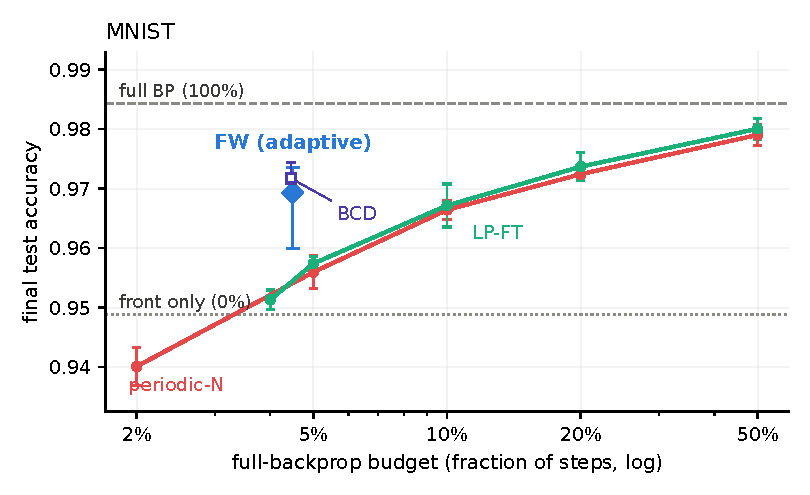
\includegraphics[width=0.82\textwidth]{exp2_pareto_mnist}
\caption{MNIST: accuracy vs.\ full-backprop budget (log scale; mean
$\pm$ std, 3 seeds). The \fw{} diamond pools all tested thresholds and
seeds---whiskers span min to max. Gray lines anchor the always-full and
never-full extremes.}
\label{fig:pareto}
\end{figure}

\begin{figure}[t]
\centering
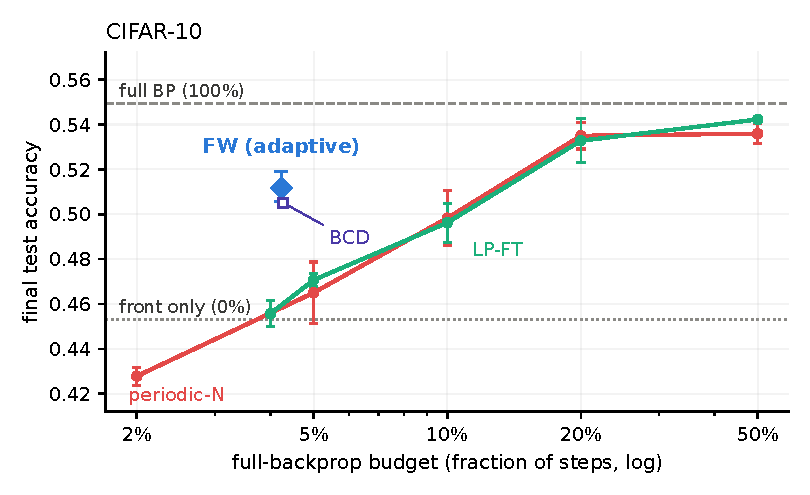
\includegraphics[width=0.82\textwidth]{exp2_pareto_cifar}
\caption{CIFAR-10: as Figure~\ref{fig:pareto}. \textsc{periodic}-$N$ and
one-switch \lpft{} trace nearly identical Pareto curves; the adaptive
schedules sit above both in the scarce-budget regime, by margins that grow
from MNIST to CIFAR-10.}
\label{fig:pareto-cifar}
\end{figure}

\paragraph{Why interleaved fixed schedules fail.} Without
gradient clipping, periodic interleaving collapsed to chance within the
first epoch on all three seeds at $N \in \{20, 50\}$, and on one of three
seeds at $N{=}10$: the front-trained, increasingly confident head
back-propagates error into a trunk it has drifted away from, with trunk
gradient norms growing to ${\sim}20\times$ their initial scale before the
collapse, driving hidden units dead. \fw{}'s \emph{consecutive} bursts
partly mitigate this (the trunk re-equilibrates within a burst), and global
norm-clipping removes it entirely; all reported runs clip at $1.0$. This is
a from-scratch analogue of the feature-distortion argument for \lpft{}
\citep{kumar2022finetuning}, here observable as a training-stability
failure rather than an out-of-distribution effect. Clipping closes the
issue under SGD; Section~\ref{sec:exp3} shows that under Adam it does not,
which is where the schedule's interaction with the optimizer becomes the
story.

\paragraph{The block choice is not the active ingredient.} \bcd{}
shares \fw{}'s closed-loop trigger but spends bursts on the complementary
block (trunk only, head frozen). It ties \fw{} on MNIST ($97.2$ vs.\
$97.1$) and trails by $1.1$ points on CIFAR-10. The scheduling mechanism
therefore transfers across block structures nearly intact; joint bursts add
a modest gain only on the harder task. Note that \bcd{} bursts cannot be
made cheap (Section~\ref{sec:framework}): only the nested scheme converts
its cheap phase into compute savings.

\paragraph{Against progressive freezing.}
The \textsc{ratchet} baseline is compared in backward compute, since its
per-step cost varies as layers freeze (its deep-step column is not
comparable; see the protocol). At matched compute, \textsc{ratchet}($0.1$)
exceeds \fw{} on MNIST consistently but not significantly ($97.3$, its own
accuracy, vs.\ \fw{}'s $97.1$; positive in all three seed pairings, $+0.22$
on average, within one seed-std), \textsc{ratchet}($0.3$) reaches $98.2$ at
a third of full BP's compute, and \fw{} leads on CIFAR-10 ($51.6$ vs.\
$50.8$ at matched compute). We therefore do not claim \fw{} beats all fixed
schedules on easy tasks; the decisive contrast appears on the transformer
(Section~\ref{sec:exp3}), where the same \textsc{ratchet}($0.1$) setting is
catastrophic---frozen-forever layers cannot recover from premature
freezing, while \fw{}'s bursts are revocable by construction.

\paragraph{Cost measurement.} We report budgets in backward
multiply--accumulates (Section~\ref{sec:framework}) because end-to-end wall
clock at this scale is dominated by the harness (data loading, kernel
launch, per-epoch evaluation): all schedules complete in ${\sim}16$s
(MNIST) / ${\sim}20$s (CIFAR-10) per run on an RTX PRO 6000. Isolated
per-step timing confirms the proxy translates once GEMMs dominate: a front
step is $1.4\times$ faster than a full step at width 512/depth 4 (batch
128), rising to $2.5$--$2.7\times$ at widths 4096--8192 and depths 8--16
(batches 512--1024), approaching the ${\sim}3\times$ limit implied by a
backward pass costing ${\sim}2\times$ the forward; the measured ratios
slightly exceed the GEMM-only prediction because the trunk's no-grad
forward also skips activation bookkeeping. Since \fw{} takes ${\sim}96\%$
front steps here, its amortized step cost approaches the front-step cost at
scale.

\section{Front wheeler on a transformer}
\label{sec:exp3}

We now change both the architecture and the optimizer: from SGD-trained
MLPs to a transformer under AdamW.

\paragraph{Conditions.} Character-level language modeling on tiny
Shakespeare: a 10.8M-parameter decoder-only transformer (6 layers,
$d{=}384$, 6 heads, context 256, dropout $0.2$), AdamW ($3{\times}10^{-4}$,
200-step warmup, cosine decay, weight decay $0.1$, clip $1.0$), 5{,}000
steps, batch 64, 3 seeds. The front is the last transformer block, the
final LayerNorm, and the LM head; the LM head is \emph{untied} from the
token embedding so front steps cannot leak trunk updates through weight
tying. Front steps run the trunk under \texttt{no\_grad}. \fw{} keeps the
MLP configuration unchanged. Metric: validation loss (lower is better);
cost: backward compute as a fraction of \textsc{full}'s. The complete
population is Table~\ref{tab:exp3matrix} (Appendix~\ref{app:tables}).

\paragraph{The low-budget result transfers.} The claim is
that \fw{}'s matched-budget advantage is not an SGD/MLP artifact.
\textsc{full} reaches $1.488 \pm 0.008$ and \textsc{front} $1.836 \pm
0.004$; \fw{} at a $6\%$ deep-step budget ($22\%$ backward compute) reaches
$1.773 \pm 0.013$---indistinguishable within seed spread from \lpft{}
spending $50\%$ of steps ($1.766 \pm 0.007$; an $8\times$ ratio in
deep-step budget, ${\sim}2.7\times$ in backward compute)---robust across
thresholds ($1.773$--$1.776$ for $\tau$ varied $10\times$), with \bcd{}
tracking at $1.797 \pm 0.010$. At matched low compute, no fixed schedule
approaches this: \lpft{}($0.95$) reaches $1.835$ and \textsc{periodic}-20
$1.910$. The gap to always-full remains substantial: \fw{} recovers
${\sim}18\%$ of the front-to-full gap here, vs.\ ${\sim}$two-thirds on
MLPs---deep trunks need more deep training on harder tasks, and \fw{}
trades quality for compute rather than matching full BP.

\begin{figure}[t]
\centering
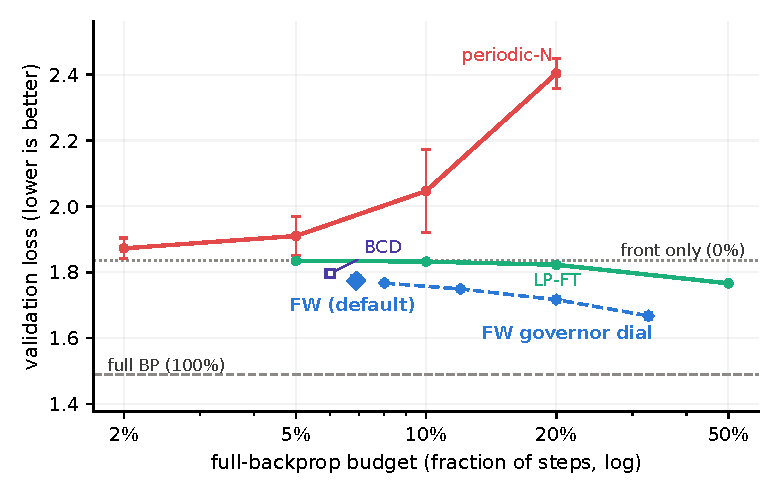
\includegraphics[width=0.72\textwidth]{exp3_pareto}
\caption{Transformer: validation loss vs.\ full-backprop budget (log
scale; mean $\pm$ std, 3 seeds; the \fw{} diamond pools thresholds,
whiskers span min to max). Periodic interleaving is
\emph{destructive}---worse than front-only at every budget, monotonically
in interleaving frequency---and one-switch \lpft{} tracks the front-only
line until half the budget is spent; at low budget, \fw{} sits below the
front-only line where one-switch and periodic schedules do not reach.}
\label{fig:exp3pareto}
\end{figure}

\paragraph{The governor is the budget dial.} Sweeping the trigger
threshold $\tau$ across two orders of magnitude ($0.005 \to 1.0$) with the
governor active barely moves the operating point: the backoff cancels eager
alarms and the budget stays pinned at $6$--$9\%$ of steps---the threshold
is a floor, not a dial. The dial is the governor itself: sweeping
$\kappa_{\max}$ from $2000$ down to $50$ traces a smooth, monotone Pareto
curve---budgets $6\% \to 49\%$ of steps, validation loss $1.773 \to
1.596$ (Figure~\ref{fig:exp3pareto})---that dominates \lpft{} and
\textsc{periodic}-$N$ at every tested budget on the transformer: at an
$8\%$ budget the dial already matches \lpft{} spending $50\%$. One
parameter selects the compute--quality operating point with no retuning of
the trigger. (On the CIFAR-10 MLP the dial's high-budget endpoint, a sweep
not reported in Section~\ref{sec:exp2}, is comparable to but does not beat
the best fixed $50\%$ schedules: $53.8$ vs.\ $54.2$ for \lpft{}.)

\paragraph{The freezing ratchet is strong but fragile.} At
\fw{}'s exact backward-compute budget, \textsc{ratchet}($0.1$) collapses to
$2.271 \pm 0.04$---worse than periodic---because it freezes five of six
blocks before the trunk has learned anything, and a ratchet cannot
un-freeze. \textsc{ratchet}($0.3$) does beat \fw{}'s default ($1.696$ vs.\
$1.773$) at $1.46\times$ the compute, and remains slightly ahead of the
\fw{} dial at matched mid-budget compute ($1.696$ at $32\%$ vs.\ $1.717$ at
$33.5\%$): a \emph{well-timed} ratchet is genuinely competitive in the
mid-budget regime. The pattern across testbeds is consistent: the ratchet's
timing is task-critical and unrecoverable when wrong, whereas \fw{} ran
identical trigger hyperparameters on every testbed in this paper.

\paragraph{Interleaving toxicity worsens under Adam.} It worsens. Periodic interleaving is destructive at every budget
tested---$1.87$ at $2\%$, worsening monotonically with interleaving
frequency to $2.40 \pm 0.05$ at a $20\%$ budget, far worse than doing
nothing deep---and it happens \emph{despite} gradient clipping, which cured
the SGD case: Adam's update $m/\sqrt{v}$ is approximately scale-invariant
in the gradient, so clipping the gradient does not clip the step. Damage
scales with interleaving \emph{frequency}, implicating repeated
perturbation---each isolated deep step moves trunk features under a head
sharply co-adapted to the old ones---and trunk moment estimates go stale
across gaps ($\beta_2 = 0.999$ means a 50-step burst refreshes only
${\sim}5\%$ of $v$), the schedule-induced analogue of the sparse-update
pathology that motivates SparseAdam for embedding tables.

\paragraph{Episodic optimizer state.}
Table~\ref{tab:optstate} is the decisive comparison, and it refined our
hypothesis. \textsc{reset-warmup} \emph{rescues} periodic interleaving
almost entirely ($2.05 \to 1.82$, from far worse than front-only to
slightly better): the dominant pathology of isolated deep steps under Adam
is stale-state re-entry at full aggression. But \textsc{reset} alone
\emph{backfires} ($2.05 \to 2.33$): a freshly initialized Adam step is the
most aggressive kind, so hygiene without gentleness is worse than
staleness. The surviving principle: \emph{the optimizer must fire with the
BP, and it must fire gently}---bursts amortize a warmup naturally, while
length-1 episodes can only approximate one by running deep steps at reduced
learning rate (for periodic, our 10-step warmup on length-1 episodes
reduces to exactly that, a caveat for interpretation). For \fw{} itself the
variants are a wash ($1.773$ persist vs.\ $1.773$ reset-warmup)---bursts
already re-equilibrate internally---which yields the systems result for
free: \emph{trunk optimizer state can be discarded between bursts at no
quality cost}, so Adam's two fp32 moments per trunk parameter need exist
only during the ${\sim}6\%$ of steps spent in bursts. The strict
\textsc{episodic} variant fails here ($2.13$), attributable to its SGD
front phases (transformers train poorly without adaptivity); a
stateless-but-adaptive front optimizer is the natural repair and is future
work.

\begin{table}[t]
\centering
\caption{Optimizer-state ablation (validation loss, mean $\pm$ std,
3 seeds). Anchors: front-only $1.836$, full BP $1.488$.}
\label{tab:optstate}
\begin{tabular}{lcc}
\toprule
Trunk Adam state & \fw{} ($6\%$) & \textsc{periodic}-10 ($10\%$) \\
\midrule
\textsc{persist} & $1.773 \pm 0.013$ & $2.047 \pm 0.127$ \\
\textsc{reset} & $1.782 \pm 0.013$ & $2.333 \pm 0.055$ \\
\textsc{reset-warmup} & $\mathbf{1.773 \pm 0.013}$ & $\mathbf{1.818 \pm 0.011}$ \\
\textsc{episodic} (SGD front) & $2.132 \pm 0.012$ & $2.437 \pm 0.008$ \\
\bottomrule
\end{tabular}
\end{table}

\subsection{Is the trigger necessary? Controls and distribution shifts}
\label{sec:controls}

Two simpler rivals could explain \fw{}'s results without any closed loop:
\textsc{ftlp} (spend all depth first, then never again) and \textsc{pburst}
(bursts on a fixed clock). We test both on the stationary task and under
two mid-training distribution shifts of different severity; complete
numbers are Tables~\ref{tab:exp3matrix} and~\ref{tab:shift}
(Appendix~\ref{app:tables}).

\paragraph{Deep-first and the fixed-cadence clock, stationary.} Only if
its one parameter is guessed correctly. At \fw{}'s matched budget,
\textsc{ftlp}($0.06$) is the worst cell in our study ($2.290 \pm 0.035$,
far below \textsc{front}): $300$ full steps from initialization---before
warmup completes---leave a half-trained trunk that is then frozen forever.
Given $3\times$ the budget, \textsc{ftlp}($0.2$) is the \emph{best} cheap
schedule we measured ($1.665 \pm 0.007$ at a $20\%$ deep-step budget).
Deep-first is a bet on knowing the right early budget: its peak and its
collapse are two settings of the same parameter. The fixed-cadence clock at
matched budget is consistently behind \fw{} ($1.814 \pm 0.014$ vs.\
$1.773 \pm 0.013$; $1.801 \pm 0.010$ with reset-warmup) though far from
failure; note its period was set \emph{from \fw{}'s own discovered
budget}---the clock is a hindsight-tuned baseline.

\paragraph{Two distribution shifts.} We switch the
training corpus mid-run at a step the schedules are not told, placed
mid-gap for \textsc{pburst}'s clock so it cannot be lucky: a \emph{mild}
shift (tiny Shakespeare $\to$ War and Peace) and a \emph{harsh} one ($\to$
C source code; the front-to-full gap grows from $0.35$ to $0.57$ of loss).
Under the mild shift \fw{} is the best cheap schedule ($1.549 \pm 0.013$),
ahead of the fair-placed clock in all three seed pairings ($1.561 \pm
0.008$), and its result is invariant to where the shift lands, which no
clock can claim; \textsc{ftlp} drops to the \textsc{front} floor ($1.605$
vs.\ $1.611$). Under the harsh shift, plain \fw{} ($1.449 \pm 0.005$)
again edges the fair-placed clock ($1.453$), while \textsc{ftlp} lands
between the floor and the burst schedules ($1.522 \pm 0.008$; its
prose-trained trunk transfers generic sequence features to code better than
a random trunk). The rivals' specific failure cells thus move with the
condition---which is itself the point: a fixed schedule's fate depends on
how well its frozen assumption happens to match the condition, and no
tested condition moved \fw{} out of the top of the cheap field or below
the \textsc{front} floor.

\paragraph{A shift-aware trigger.} \fw{}'s
documented weakness is that the backoff, stretched long by pre-shift
saturation, delays post-shift re-escalation (mild shift: $12\%$ of the
front-to-full gap recovered, vs.\ $18\%$ stationary). The repair is one
line: reset the cooldown when the loss EMA \emph{jumps above} its running
minimum---a shift signature, the opposite of the plateau the trigger
watches for. Under the harsh shift this \emph{governor reset} responds by
spending $6.7\%$ deep steps (vs.\ plain \fw{}'s $4\%$; the budget is
self-selected) and reaches $1.411 \pm 0.005$---the best cheap schedule
under the hardest condition we tested, recovering $24\%$ of the
front-to-full gap vs.\ plain \fw{}'s $18\%$. The trigger's verdict across
every test, stated at full strength and no more: bursts carry the
performance; a fixed clock, its period set with hindsight, ties or
slightly trails \fw{}; the closed loop's demonstrated products are
discovering the schedule without that hindsight, robustness when
assumptions break, and---with the one-line reset---responsiveness to them
breaking.

\paragraph{Measured resources validate the cost model---with one caveat.}
End-to-end single runs (2{,}000 steps, identical hardware;
Appendix~\ref{app:infra}) measure: full BP $98.4$s, \fw{} $49.3$s,
\textsc{ratchet}($0.1$) $49.7$s, front-only $46.6$s---\fw{} and the
compute-matched ratchet are equal-cost in wall clock to within $1\%$, and
\fw{} delivers a real $2.0\times$ end-to-end speedup over full BP at this
scale (per-step: $23.3$ms front vs.\ $49.2$ms full). The caveat is peak
activation memory: front-only peaks at $0.77$\,GB, but any schedule that
ever takes a full-depth step---\fw{} included---peaks at $3.03$\,GB,
because the peak is set by the deepest single step. \fw{} reduces
\emph{average} memory and (via episodic state) trunk optimizer memory, not
the activation peak; activation checkpointing inside bursts, which are
only ${\sim}6\%$ of steps, is the natural remedy and is future work.

\noindent The results so far take the premise---that cheap front steps
carry most per-step progress---as given; the experiments that supplied it
are reported in Appendix~\ref{sec:exp1}.

\section{Origins: the wiring experiments that motivated front wheeler}
\label{sec:exp1}

\fw{} rests on a premise: most per-step improvement does not require deep
credit assignment. The experiments in this section---originally aimed at a
different question---supplied that premise. Supermask results show that a
randomly weighted, sufficiently wide network already contains subnetworks
that solve the task \citep{ramanujan2020whats, zhou2019deconstructing,
malach2020proving}; we asked how \emph{local} the search for such a
subnetwork can be made, and the control conditions of that study are what
pointed at \fw{}.

\paragraph{Setup.} MLPs with frozen random weights (signed-constant
initialization); only a binary mask (top-$k$ scores per layer, $50\%$ kept)
is learned. Rules, ordered by the information available to hidden layers:
\ep{} (straight-through gradients on scores, i.e.\ full BP---the upper
bound), \dfa{} (the layer's error is a fixed random projection of the output
error \citep{nokland2016direct}, applied here to mask scores: no weight
transport, no chained backward), and \rmhebb{} (hidden layers see one global
scalar per sample modulating a batch-centered Hebbian eligibility
\citep{fremaux2016neuromodulated, williams1992simple}). Controls:
\textsc{random} mask, \textsc{readout} (train the final layer only), and
\textsc{dense} (ordinary training). 30/40 epochs (MNIST/CIFAR-10), 3 seeds.

\begin{table}[t]
\centering
\caption{Final test accuracy (mean $\pm$ std, 3 seeds), at two and four
hidden layers. Only the mask is learned in \ep{}/\dfa{}/\rmhebb{}.}
\label{tab:exp1}
\begin{tabular}{lcccc}
\toprule
& \multicolumn{2}{c}{2 hidden layers} & \multicolumn{2}{c}{4 hidden layers} \\
Rule & MNIST & CIFAR-10 & MNIST & CIFAR-10 \\
\midrule
\textsc{dense} (control) & $98.7 \pm 0.1$ & $53.0 \pm 0.4$ & --- & --- \\
\ep{} & $98.2 \pm 0.1$ & $\mathbf{55.9 \pm 0.2}$ & $98.3 \pm 0.1$ & $\mathbf{56.2 \pm 0.1}$ \\
\dfa{} & $96.9 \pm 0.1$ & $53.3 \pm 0.2$ & $81.8 \pm 0.9$ & $23.1 \pm 8.9$ \\
\textsc{readout} (control) & $94.9 \pm 0.1$ & $45.6 \pm 0.2$ & --- & --- \\
\rmhebb{} & $51.7 \pm 3.9$ & $26.3 \pm 6.3$ & $34.1 \pm 9.9$ & $18.2 \pm 4.0$ \\
\textsc{random} (control) & $12.5 \pm 3.5$ & $10.1 \pm 0.8$ & --- & --- \\
\bottomrule
\end{tabular}
\end{table}

\paragraph{What holds, and what is shallow-only.} Three results
(Table~\ref{tab:exp1}, Figure~\ref{fig:exp1curves}). First, \emph{wiring
rivals weights, robustly}: gradient mask search over frozen random weights
comes within half a point of dense training on MNIST, beats it on CIFAR-10
($55.9\%$ vs.\ $53.0\%$, where the dense MLP overfits), and is
depth-stable---at four hidden layers it is unchanged or better. Second,
\emph{the local rule's parity is a shallow-network phenomenon}: at two
hidden layers \dfa{} mask search matches dense weight training on CIFAR-10,
but at four hidden layers it collapses ($96.9 \to 81.8$ on MNIST,
$53.3 \to 23.1$ with large seed variance on CIFAR-10), consistent with
feedback alignment's known depth pathology. Claims about local wiring rules
in this paper are therefore scoped to shallow networks. Third, \emph{a
global scalar is not enough at any depth we tested}: \rmhebb{} stays far
below every vector-signal rule and degrades further with depth. Mask-budget
robustness at two hidden layers is shown in Figure~\ref{fig:sparsity}.

\paragraph{The observation that led to \fw{}.} The \textsc{readout} control
is the quiet protagonist: training \emph{only the top} of a frozen random
network already recovers $94.9\%$ on MNIST and $45.6\%$ on CIFAR-10---most
of the accuracy of full training, for a small fraction of its backward
cost. If cheap top-only updates carry that much of the signal, full-depth
credit assignment is needed only occasionally, and the question becomes
\emph{when}: the scheduling problem \fw{} answers.

\begin{figure}[t]
\centering
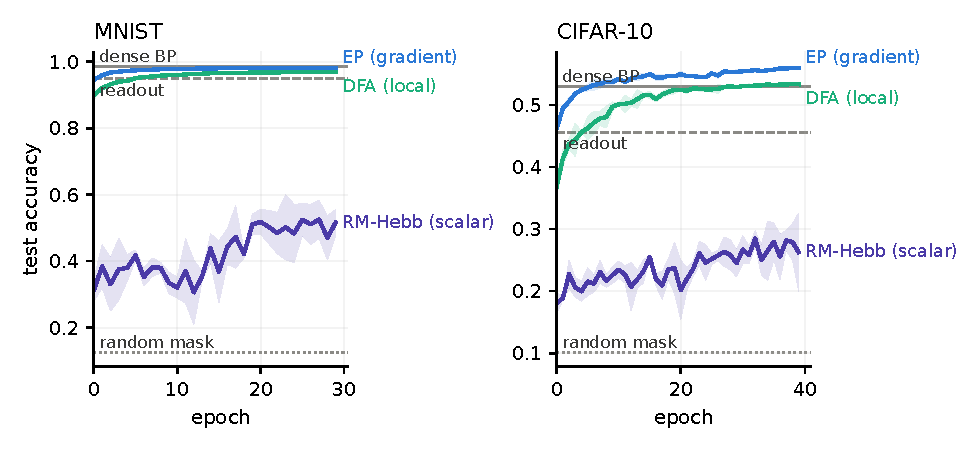
\includegraphics[width=\textwidth]{exp1_locality}
\caption{Learning curves for the wiring rules at two hidden layers (mean
over 3 seeds; bands $\pm 1$ std). Colored curves learn only the mask over
frozen random weights; gray lines mark the controls. At this depth the
vector-signal rules (\ep{}, \dfa{}) finish within two points of dense
training or above it; Table~\ref{tab:exp1} shows \dfa{}'s parity does not
survive depth 4.}
\label{fig:exp1curves}
\end{figure}

\begin{figure}[t]
\centering
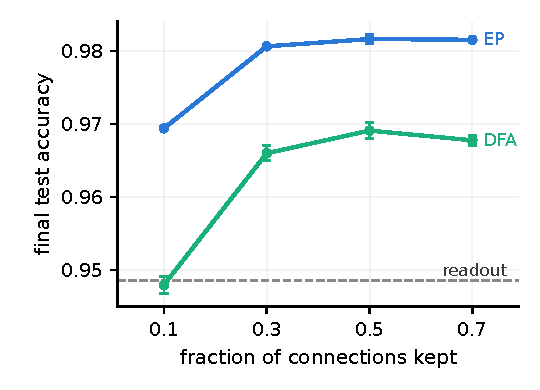
\includegraphics[width=0.5\textwidth]{exp1_sparsity}
\caption{Mask-budget robustness on MNIST (2 hidden layers): both search
rules degrade gracefully down to $10\%$ of connections kept, where the local
rule still matches the trained-readout control.}
\label{fig:sparsity}
\end{figure}

\subsection{Two failure modes worth documenting}
\label{sec:exp1-stability}

\paragraph{The sign factor in straight-through mask gradients.} Selecting the
top-$k$ mask by $|s|$ while passing the straight-through gradient to $s$
directly drops the $\partial|s|/\partial s = \operatorname{sign}(s)$ factor;
every negative-score synapse then moves in the wrong direction, and learning
sits at chance. Applying $|\cdot|$ \emph{before} the straight-through
operator (so autodiff supplies the sign), or equivalently multiplying manual
updates by $\operatorname{sign}(s)$, restores learning entirely. We flag this
because the failure is silent: losses hover near initialization and no error
is raised.

\paragraph{Hebbian runaway and its stabilization.} A naive three-factor rule
diverges here: with ReLU activity the eligibility $a_i x_j$ is non-negative,
so reinforced co-activations grow activations, which grow eligibilities,
until logits saturate (magnitudes ${>}10^2$ within 200 steps), the softmax
collapses to one-hot, exploration dies, and accuracy pins at chance.
Batch-centered (covariance) eligibilities, RMS-normalized per-layer updates,
and a loss-based rather than sampled-action reward stabilize it; the
stabilized rule learns but remains far below the vector-signal rules.

\section{Discussion and limitations}
\label{sec:discussion}

\paragraph{One question, two axes.} Both experiments degrade the same
resource---globally informed, per-step credit assignment---along orthogonal
axes. Axis~1 fixes \emph{when} (every step) and varies \emph{what} each
synapse may know; the answer is that connectivity search survives the loss of
weight transport and the chained backward (\dfa{}), and fails gracefully but
substantially when compressed to a scalar (\rmhebb{}). Axis~2 fixes
\emph{what} (exact gradients) and varies \emph{when} depth is paid for; the
answer is that ${\sim}4\%$ of steps, placed adaptively, recover roughly
two-thirds of the accuracy gap between never and always paying for
depth---and that among the schedules we tested at that budget, only the
adaptive ones do. In both cases the interesting quantity is not the best
achievable accuracy but the \emph{shape of the degradation}: graceful along
locality until the vector-to-scalar cliff, graceful along frequency provided
the schedule is closed-loop.

\paragraph{What we do not claim.} All experiments use MLPs on MNIST and
CIFAR-10 with three seeds; absolute accuracies are far from competitive, by
design. We make no claim that these orderings persist in convolutional or
attention-based architectures, at scale, or under distribution shift. The
per-step timing model transfers to transformers only in outline (a
last-block-plus-head front step has the same structure, but attention
backward and activation memory change the constants). The \rmhebb{} result
in particular bounds only the specific three-factor rule we stabilized; a
better scalar-modulated rule may exist, and our finding should be read as
``the obvious one is insufficient,'' not as an impossibility result.

\paragraph{What we believe transfers.} Three mechanisms, not the numbers:
(i)~the cost asymmetry of nested versus partitioned blocks---depth truncation
is exclusive to the top block, so compute-aware scheduling should treat block
choice and burst timing as separate decisions; (ii)~burst-as-measurement with
backoff---any scheduler that must decide whether expensive credit assignment
is still productive faces the cried-wolf problem, and exponential backoff is
a simple, robust answer; (iii)~the danger of isolated deep steps into a stale
trunk, which links training stability to the \lpft{} feature-distortion
mechanism and predicts that interleaved partial-training schemes need either
burst structure or gradient clipping.

\paragraph{Open directions.} Making the trigger's implicit estimate of
inequality~\eqref{eq:greedy} explicit (e.g., cheap stochastic probes of
$\|\nabla L\|$) would turn \fw{} from a heuristic into an approximate optimal
stopping rule. On Axis~1, the gap between \dfa{} and \ep{} may close with
layer-wise mask budgets or momentum on scores; and the vector-to-scalar cliff
invites a controlled study of intermediate signals (low-rank error sketches,
per-class scalars) to locate the threshold precisely.

\section{Conclusion}
Random networks already contain their solutions; finding them does not
require backpropagation's full machinery---an error broadcast suffices---but
it does require more than the scalar-modulated rule we could stabilize. And
when exact gradients are available, most steps do not need them: a
plateau-triggered controller with backoff spends $4\%$ of the depth budget to
recover about two-thirds of the accuracy gap between never and always paying
for it, and beats every fixed alternative we tested at that budget. Both results argue that
credit assignment is best understood as a budgeted resource with structure in
\emph{where} and \emph{when} it is spent, not a fixed per-step cost.

\paragraph{Reproducibility.} Code, run logs, and all raw result CSVs are
available at \url{https://github.com/XTAM-AI/front-wheeler}. Every number in this paper is the
mean over seeds $\{0,1,2\}$ with the exact commands recorded in the run
scripts.


\section*{Acknowledgments}
This work was carried out at XTAM Research Labs. Transparency about tooling:
this work was AI-assisted (Anthropic's Claude---Claude Code, Claude Fable
5---for implementation, experiment orchestration, debugging, and drafting),
under the direction and review of the author. All results were produced by
the released code, and every reported number was checked against the raw run
logs in the repository.

\bibliographystyle{unsrtnat}
\bibliography{refs}

\appendix

\section{Experimental infrastructure}
\label{app:infra}
All experiments ran on a single workstation: one NVIDIA RTX PRO 6000
Blackwell (96\,GB), 64 CPU cores, 256\,GB RAM; PyTorch 2.13 / CUDA~13 in a
micromamba environment. The complete experimental suite---both MLP studies,
the transformer study, and all ablations and sweeps, three seeds
throughout---consumes under ten GPU-hours end to end. Datasets: MNIST
\citep{lecun1998gradient}, CIFAR-10 \citep{krizhevsky2009learning}, and the
tiny Shakespeare corpus. Exact commands for every run are recorded in the
repository's \texttt{scripts/} directory; per-run CSV logs (including
wall-clock times) are in \texttt{results/}.

\section{Two failure modes of mask-search rules}
\label{app:failures}

\paragraph{The sign factor in straight-through mask gradients.} Selecting the
top-$k$ mask by $|s|$ while passing the straight-through gradient to $s$
directly drops the $\partial|s|/\partial s = \operatorname{sign}(s)$ factor;
every negative-score synapse then moves in the wrong direction, and learning
sits at chance. Applying $|\cdot|$ \emph{before} the straight-through
operator (so autodiff supplies the sign), or equivalently multiplying manual
updates by $\operatorname{sign}(s)$, restores learning entirely. We flag this
because the failure is silent: losses hover near initialization and no error
is raised.

\paragraph{Hebbian runaway and its stabilization.} A naive three-factor rule
diverges here: with ReLU activity the eligibility $a_i x_j$ is non-negative,
so reinforced co-activations grow activations, which grow eligibilities,
until logits saturate (magnitudes ${>}10^2$ within 200 steps), the softmax
collapses to one-hot, exploration dies, and accuracy pins at chance.
Batch-centered (covariance) eligibilities, RMS-normalized per-layer updates,
and a loss-based rather than sampled-action reward stabilize it; the
stabilized rule learns but remains far below the vector-signal rules.

\end{document}
